\documentclass[]{article}
\usepackage{graphicx}
%opening
\title{Software Requirement Specification Document}
\author{Mariam Hesham,Nour Ahmed ,Samiha Hesham, Sandra Fares }

\begin{document}

\maketitle

\section{Introduction}

\subsection{Purpose of this document}
The main purpose of this document is to clarify and demonstrate the requirements of a Clinic System. These requirements include booking appointments, contacting Doctors or Physician assistants, and viewing patients' medical information. Our aim is to assist patients' to reserve appointments and reach out to healthcare professionals easily. Moreover, our system shall make it easier for Doctors to view patients' medical information, in order to provide accurate diagnosis. This documentation shall provide an explanation of each phase, along with an illustration on how this system is going to function. 

\subsection{ Scope of this document}
The scope of this document is to break down our client's problems into chunks that can be solved more readily.It also helps to increase understanding of issues and makes them easier to be tackled through our system and tested properly to fulfil the optimum solutions. 


\subsection{Overview}
Provides a brief overview of the product defined as a result of the requirements elicitation process. 


\section{General Description}

\subsection{Product Functions}
\begin{enumerate}
  \item The system must be fully dynamic,in which the admin is fully controlling the system
  \item The users(patients,doctor,receptionists,assistants) must be able to control their information 
  \item The patient must be able to reserve his/her appointment online and choose either paying online or cash.
  \item The system should be able to send automatic emails and SMS to the patients.
  \item The admin should have full authority to control all staff permissions.
  \item The doctor must be able to see full information of the patient.
  \item The doctor should has the ability to write a report to the patient's case with all details.
  \item The doctor must be able to reserve operation for the patient if needed.
  \item The assistant must organize the doctor's schedule and add,edit or delete operations to it.
  \item The assistant should perform a broadcast en-forming patients of any cancellation in the doctor's schedule.
  \item The patients must have the authority to edit their appointment details.
  \item The receptionist must view patients' reservations and should deal with financial staff.
\end{enumerate}

\subsection{Similar System Information}
This software is similar to various generic products. However, MedDNA and eClinic are the most similar to our system. These systems are stand-alone clinic management systems that are available for installation by any customer in need. Their purpose is to help in managing appointments, viewing patients' history, and offering effortless communication between the Doctors and their Patients, just like our system is intended to do.


\subsection{ User Characteristics}
The admin, doctor, receptionists, assistants and patients will be the main users. The system is also designed to be user-friendly. 

\begin{itemize}
  \item Admin
  \item Receptionists
  \item Doctor
  \item Assistants
  \item Patients
  
  
\end{itemize}

Admin: Admin should have prior knowledge of the system. Admin is able to control the whole system. He/she can add, delete, update and modify the system.


Receptionists: in order view the details of the patients come for the treatment and accordingly provides identity to them also, schedule the appointments of the day and deals with payment methods. 


Doctor: Doctor should fairly know about the usage of the system. Doctor are able to see the respective appointments taken. And also, can view patient’s details and records and set for them operations if needed.


Assistants: they are mainly managing the chatting system for the clinic with patients and they must  view, edit ,delete and add operations in the doctor’s schedule.


Casual users: Anyone can view the information of the polyclinic. Patients can view their own records and doctor’s details and timings to take appointment online.


\subsection{ User Problem Statement}
This section describes the essential problem(s) currently confronted by the user community. 

\section{Functional Requirements}
This section lists the functional requirements in ranked order. Functional requirements describes the possible effects of a software system, in other words, what the system must accomplish. Other kinds of requirements (such as interface requirements, performance requirements, or reliability requirements) describe how the system accomplishes its functional requirements. Each functional requirement should be specified in a format similar to the following: 
1.	Short, imperative sentence stating highest ranked functional requirement.
1.	Description
A full description of the requirement. 
2.	Criticality
Describes how essential this requirement is to the overall system. 
3.	Technical issues
Describes any design or implementation issues involved in satisfying this requirement. 
4.	Cost and schedule
Describes the relative or absolute costs associated with this issue. 
5.	Risks
Describes the circumstances under which this requirement might not able to be satisfied, and what actions can be taken to reduce the probability of this occurrence. 
6.	Dependencies with other requirements
Describes interactions with other requirements. 
7.	... others as appropriate
2.	<Name of second highest ranked requirement>
And so forth... 

\section{Interface Requirements}
This section describes how the software interfaces with other software products or users for input or output. Examples of such interfaces include library routines, token streams, shared memory, data streams, and so forth. 

\subsection{User Interfaces}
Use some software for primitive plan of your project.
Describes how this product interfaces with the user. 

\subsubsection {GUI}
Describes the graphical user interface if present. This section should include a set of screen dumps or mockups to illustrate user interface features. 
If the system is menu-driven, a description of all menus and their components should be provided. 

\subsubsection { CLI}
Describes the command-line interface if present. For each command, a description of all arguments and example values and invocations should be provided. 

\subsection {API}
Describes the application programming interface, if present. For each public interface function, the name, arguments, return values, examples of invocation, and interactions with other functions should be provided. 

\section{Design Constraints}
Specifies any constraints for the design team using this document. 

\section{Other non-functional attributes}
Specifies any other particular non-functional attributes required by the system. Examples are provided below. 

\subsection {Security}
This system is provided with authentication without which no user can pass. So only the legitimate users are allowed to use the application. If the legitimate user’s share the authentication information then the system is open to outsiders.



\subsection {Reliability}
Good validations of user inputs will be done to avoid incorrect storage of records.
\subsection {Maintainability}
\subsection {Portability}
This system can be installed in any personal computers supporting windows operating system platform.
\subsection {Flexibility}
The system keeps on updating the data according to the transactions that takes place.

\section{Preliminary Object-Oriented Domain Analysis}
This section presents a list of the fundamental objects that must be modeled within the system to satisfy its requirements. The purpose is to provide an alternative, ''structural'' view on the requirements stated above and how they might be satisfied in the system. A primitive class diagram to be delivered.

\subsection{Inheritance Relationships}
This section should contain a set of graphs that illustrate the primary inheritance hierarchy (is-kind-of) for the system. For example: 

\begin{figure}[tbh]
\centering
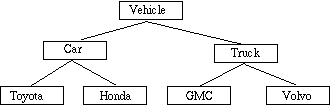
\includegraphics[width=0.7\linewidth]{./image}
\caption{Inheritance Relations}
\label{fig:image}
\end{figure}

\subsection{Class descriptions}
This section presents a more detailed description of each class identified during the OO Domain Analysis.
Each class description should conform to the following structure: 

\begin{table}[h]
\caption{Class Name - }
\label{tab:my-table}
\begin{tabular}{|p{0.25\textwidth}|p{0.75\textwidth}|}
\hline
\textbf{Abstract or Concrete:} & Indicates whether this class is abstract or concrete.
\\ \hline
\textbf{List of Superclasses}  & Names all immediate superclasses.                                                       
\\ \hline
\textbf{List of Subclasses}    & List of Subclasses                                                                      
\\ \hline
\textbf{Purpose}               & Purpose                                                                                 
\\ \hline
\textbf{Collaborations}        & Names each class with which this class must interact in order to accomplish its purpose, and how.
\\ \hline
\textbf{Attributes}            & Lists each attribute (state variable) associated with each instance of this class, and indicates examples of possible values (or a range).
\\ \hline
\textbf{Operations}            & Lists each operation that can be invoked upon instances of this class.  For each operation, the arguments (and their type), the return value (and its type), and any side effects of the operation should be specified. 
\\ \hline
\textbf{Constraints}           & Lists any restrictions upon the general state or behavior of instances of this class.   
\\ \hline
\end{tabular}
\end{table}

\section{Operational Scenarios}
This section should describe a set of scenarios that illustrate, from the user's perspective, what will be experienced when utilizing the system under various situations. 
In the article Inquiry-Based Requirements Analysis (IEEE Software, March 1994), scenarios are defined as follows: 
In the broad sense, a scenario is simply a proposed specific use of the system. More specifically, a scenario is a description of one or more end-to-end transactions involving the required system and its environment. Scenarios can be documented in different ways, depending up on the level of detail needed. The simplest form is a use case, which consists merely of a short description with a number attached. More detailed forms are called scripts. These are usually represented as tables or diagrams and involved identifying an action and the agent (doer) of the action. FOr this reason, a script can also be called an action table. 
Although scenarios are useful in acquiring and validating requirements, they are not themselves requirements, because the describe the system's behavior only in specific situations; a specification, on the other hand, describes what the system should do in general. 

\section{Project Plan}
This section provides an initial version of the project plan, including the major tasks to be accomplished, their interdependencies, and their tentative start/stop dates. The plan also includes information on hardware, software, and  resource requirements. 
The project plan should be accompanied by one or more PERT or GANTT charts. 

\section{Appendices}
Specifies other useful information for understanding the requirements. All SRS documents should include at least the following two appendices: 

\subsection{Definitions, Acronyms, Abbreviations}
Provides definitions of unfamiliar definitions, terms, and acronyms. 

\subsection{Collected material}

\section {References}

\bibliographystyle{IEEEtranS}

\bibliography{cite}

\end{document}
